\documentclass{beamer}

\usepackage[applemac]{inputenc}
\usepackage{latexsym}
\usepackage{graphicx}
\usepackage[english]{babel}
\usepackage{amsmath,amssymb}
\usepackage{calc}
\usepackage{multicol}
\usepackage{fancyhdr}
\usepackage{lastpage}
\usepackage[T1]{fontenc}
\usepackage{lmodern}
\usepackage{stmaryrd}
\usepackage{float}
\usepackage{textcomp}
\usepackage{tikz}  



\setbeamertemplate{footline}[frame number] 
\usetheme{Madrid}


\beamertemplatenavigationsymbolsempty


% \usepackage{beamerthemesplit} // Activate for custom appearance

\title{ADVANCED LEARNING FOR TEXT AND GRAPH DATA \\ Final Project: Text categorization}
\author{Mathurin \textsc{Massias} \and Cl�ment \textsc{Nicolle} \and Micha�l \textsc{Weiss}}
\date{\today} 



\begin{document}


\frame{\titlepage}


\frame
{
  \frametitle{Problem setup}
  \begin{itemize}
	  \item Multi-label text classification problem
	  \item 5,485 documents for training
 	 \item 2,189 documents for testing
  \end{itemize}
}

\frame
{
	\frametitle{Performance evaluation}
	 \begin{itemize}
	  	\item Classification performance: precision and recall
		  \item Micro and macro averaging
 		 \item Training time
		 \item Prediction time
 	 \end{itemize}

}

\frame
{
	\frametitle{Algorithms used}	
	 \begin{itemize}
	  	 \item k Nearest neighbors
		  \item Multi label SVM (one vs one)
		  \item Random Forest
		 \item Adaboost
 	 \end{itemize}	
}

\frame
{
	\frametitle{Algorithms used}
	Parameters estimation ?
	\begin{itemize}
		\item k 
		\item $C$, $\gamma$ 
		\item Number of trees
		\item Number of weak learners
	\end{itemize}
	Cross validation: split the training set, train on one part, evaluate on the other.
	Performance criterion: micro-averaging precision/recall.
}

\frame
{
	\frametitle{Cross-validation}
  \begin{figure}[H]
  	\centering
  	\noindent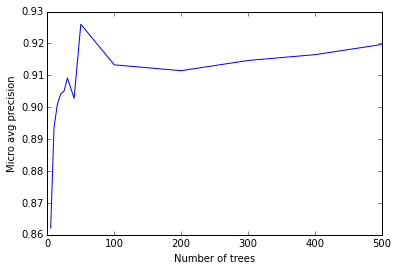
\includegraphics[scale=0.5]{CV_RF.png}
	\caption{Micro averaging error as a function of the number of trees for Random forest}
  \end{figure}
  }

\frame
{
	\frametitle{Features used}	
	 \begin{itemize}
	  	 \item Bag of words model
		  \item Graph of words (unweighted edges)
		  \item Graph of words (weighted edges)
 	 \end{itemize}	
}


\frame
{
	\frametitle{Results: bag of words}	
	
	\begin{table}[h]
          \begin{tabular}[scale=0.1]{|l|c|c|c|c|}
		\hline
		\multicolumn{1}{|c|}{Algorithm \textbackslash Performance} & \begin{tabular}[c]{@{}c@{}}Micro-averaging\\ precision/recall\end{tabular} & \begin{tabular}[c]{@{}c@{}}Macro-averaging\\ precision\end{tabular} & \begin{tabular}[c]{@{}c@{}}Macro-averaging\\ recall\end{tabular} & Training time \\ \hline
		k-NN                                        & 84.42\%                                                                    & 85.40\%                                                             & 82.74\%                                                          & 1543 s           \\ \hline
		SVM                                         & 89.31\%                                                                    & 92.63\%                                                             & 65.06\%                                                          & 1021 s           \\ \hline
		Random Forest                               & 91.6\%                                                                     & 89.46\%                                                             & 62.84\%                                                          & 7 s           \\ \hline
		Adaboost                                    & 79.1\%                                                                    & 57.02\%                                                             & 57.86\%                                                          & 204 s           \\ \hline
	\end{tabular}
	\caption{Time and classification performance for various algorithms on the bag-of-words model}
	\end{table}
}

\frame
{
	\frametitle{Results: graph of words (unweighted)}	
	Which centrality measure ?
	\begin{itemize}
	\item Degree centrality measure?
	\item Eigenvector centrality measure?
	\end{itemize}
}

\frame
{
	\frametitle{Results: graph of words (unweighted)}	
	
	\begin{table}[H]
	\begin{tabular}{|l|c|c|c|}
		\hline
		\multicolumn{1}{|c|}{Algorithm \textbackslash Performance} & \begin{tabular}[c]{@{}c@{}}Micro-averaging\\ precision/recall\end{tabular} & \begin{tabular}[c]{@{}c@{}}Macro-averaging\\ precision\end{tabular} & \begin{tabular}[c]{@{}c@{}}Macro-averaging\\ recall\end{tabular} \\ \hline
		k-NN                                        & 86.16\%                                                                    & 83.64\%                                                             & 82.22\%           \\ \hline
		SVM                                         & 95.16\%                                                                    & 95.44\%                                                             & 79.89\%            \\ \hline
		Random Forest                               & 91.09\%                                                                     & 86.05\%                                                             & 66.07\%             \\ \hline
		Adaboost                                    & 79.53\%                                                                    & 67.18\%                                                             & 67.36\%              \\ \hline
	\end{tabular}
	\caption{Classification performance by algorithm for Degree Centrality measure}
\end{table}
}


\frame
{
	\frametitle{Results: graph of words (unweighted)}	
\begin{table}[H]
	\begin{tabular}{|l|c|c|c|}
		\hline
		\multicolumn{1}{|c|}{Algorithm \textbackslash Performance} & \begin{tabular}[c]{@{}c@{}}Micro-averaging\\ precision/recall\end{tabular} & \begin{tabular}[c]{@{}c@{}}Macro-averaging\\ precision\end{tabular} & \begin{tabular}[c]{@{}c@{}}Macro-averaging\\ recall\end{tabular} \\ \hline
		k-NN                                        & 86.71\%                                                                    & 82.53\%                                                             & 81.91\%           \\ \hline
		SVM                                         & 93.24\%                                                                    & 94.11\%                                                             & 69.66\%            \\ \hline
		Random Forest                               & 91.65\%                                                                     & 88.95\%                                                             & 68.47\%             \\ \hline
		Adaboost                                    & 79.03\%                                                                    & 66.49\%                                                             & 60.98\%              \\ \hline
	\end{tabular}	
	\caption{Classification performance by algorithm for Eigenvector Centrality measure}

\end{table}
}


\frame
{
	\frametitle{Results: graph of words (weighted)}	
	
	\begin{table}[H]
	\begin{tabular}{|l|c|c|c|}
		\hline
		\multicolumn{1}{|c|}{Algorithm \textbackslash Performance} & \begin{tabular}[c]{@{}c@{}}Micro-averaging\\ precision/recall\end{tabular} & \begin{tabular}[c]{@{}c@{}}Macro-averaging\\ precision\end{tabular} & \begin{tabular}[c]{@{}c@{}}Macro-averaging\\ recall\end{tabular} \\ \hline
		k-NN                                        & 86.25\%                                                                    & 86.96\%                                                             & 81.55\%           \\ \hline
		SVM                                         & 95.25\%                                                                    & 95.38\%                                                             & 79.62\%            \\ \hline
		Random Forest                               & 91.82\%                                                                     & 90.58\%                                                             & 69.33\%             \\ \hline
		Adaboost                                    & 79.21\%                                                                    & 69.01\%                                                             & 65.97\%              \\ \hline
	\end{tabular}
	\caption{Classification performance by algorithm for Weighted Edges with Degree Centrality measure}
\end{table}
}



\frame
{
	\begin{center}
		Thank you for your attention
	\end{center}
}


\end{document}
